% !TEX root = ../paper.tex

\section{Evaluation}

This section describes the result of the empiric evaluation of both described algorithms.

\subsection{Single-Writer-Multi-Reader Lock Implementation}

For conducting the expiriments a Sun SPARC T5240 was used, which consists of two UltraSPARC T2 Plus chips with 8 cores each, running at 1.165~GHz. Each core provides 8 hardware threads, for a total of 128 threads (64 per chip).

\improve{Criticise why use this machine? seems quite old? why no more threads? why hide compiler details and os? why not all evaluate on the Intel machine?}

\begin{figure}[htb]
	\centering
	\begin{minipage}[b]{.495\textwidth}
		\centering
		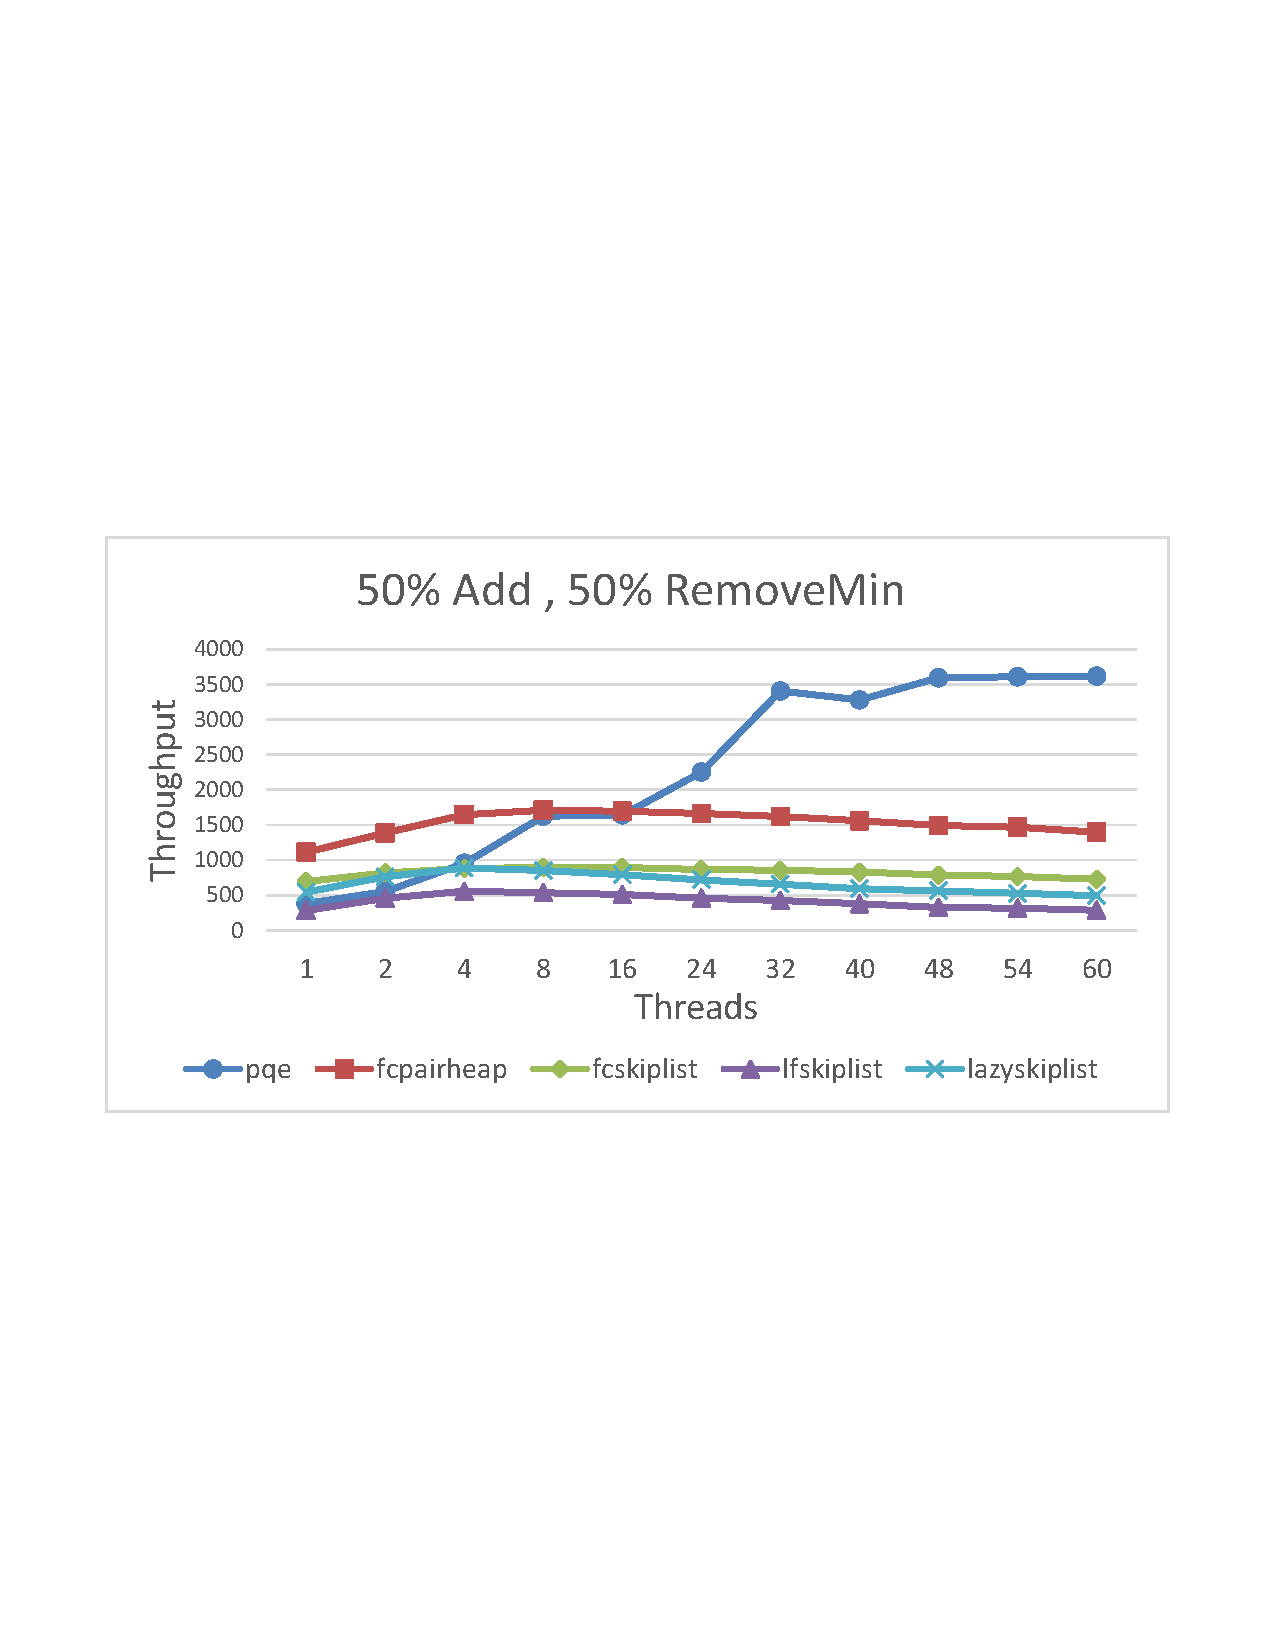
\includegraphics[width=\linewidth]{graphics/sparc-50-50.pdf}
		\caption{Priority queue performance with 50\% \texttt{add()}s, 50\% \texttt{removeMin()}s \cite{calciu_adaptive_2014}.}
		\label{fig:sparc_50}
	\end{minipage}
	\hfill%
	\begin{minipage}[b]{.495\textwidth}
		\centering
		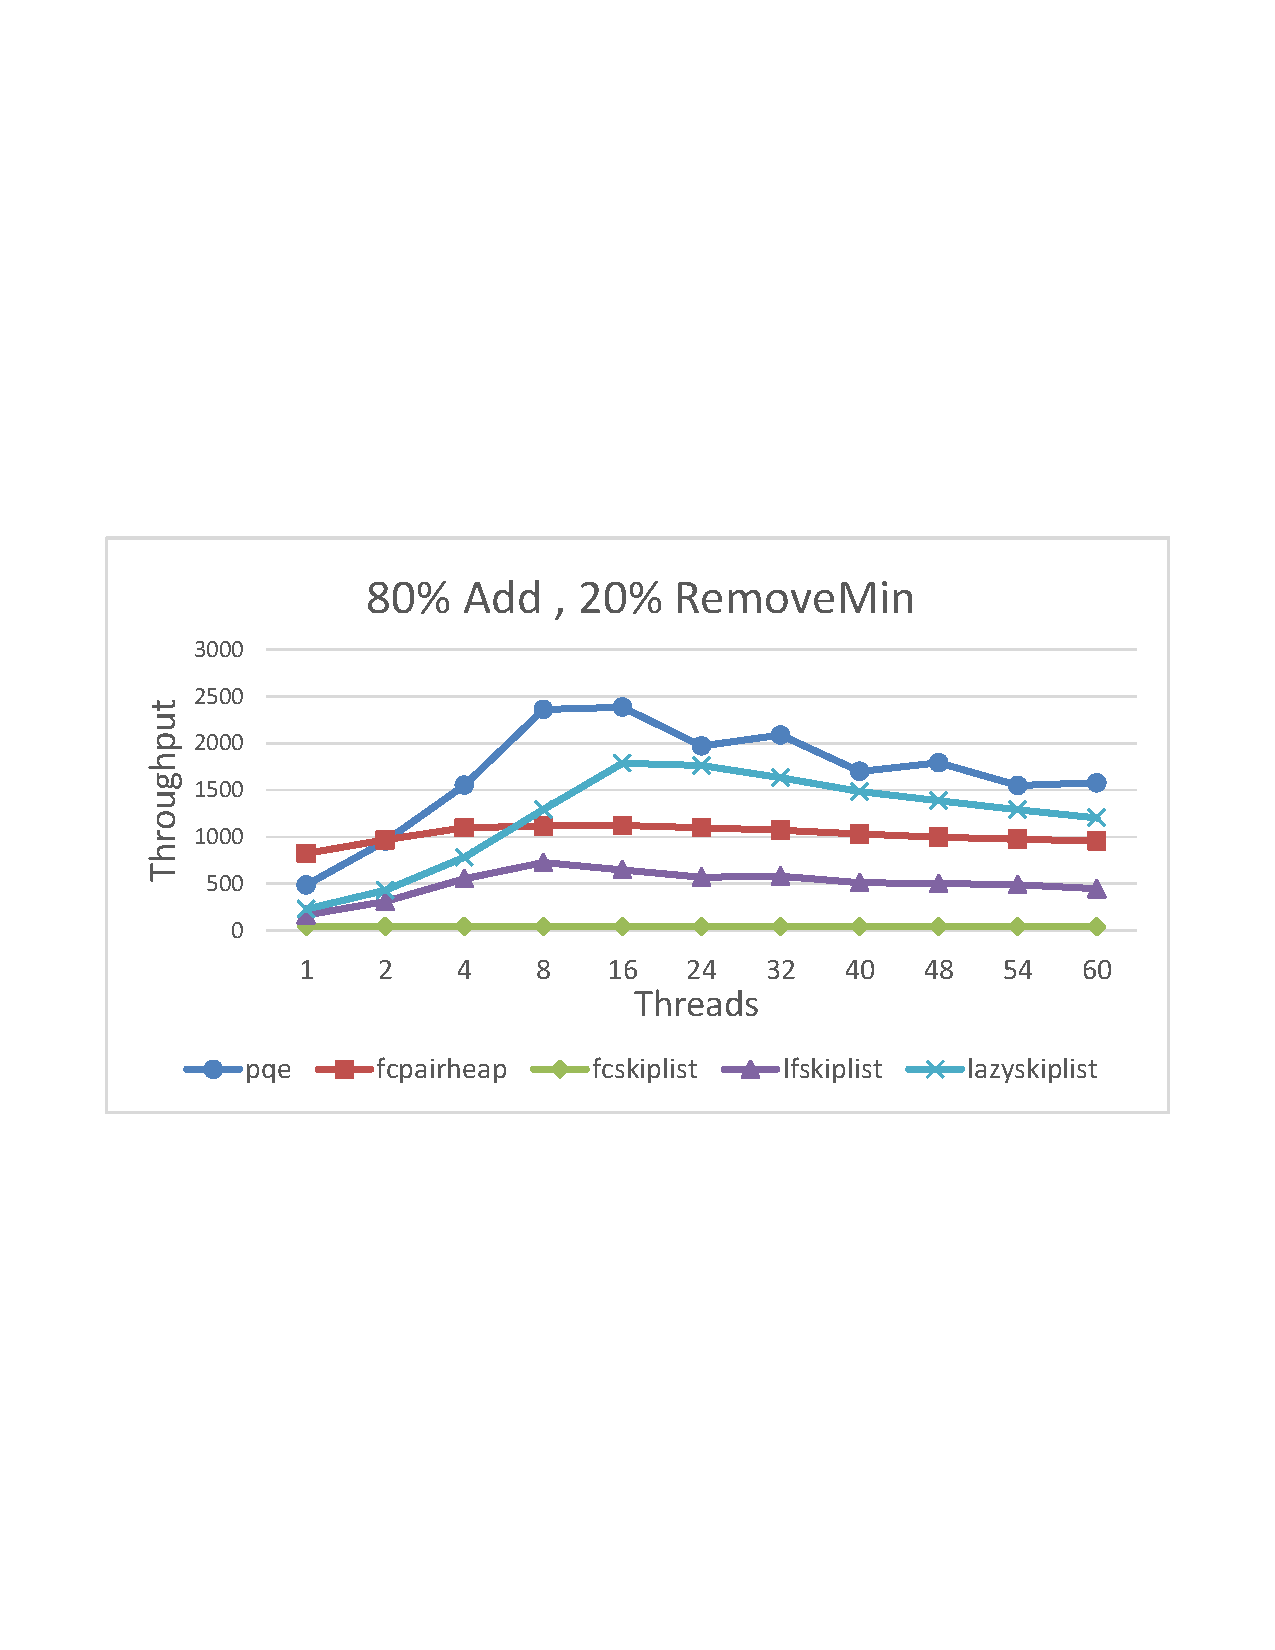
\includegraphics[width=\linewidth]{graphics/sparc-80-20.pdf}
		\caption{Priority queue performance with 80\% \texttt{add()}s, 20\% \texttt{removeMin()}s \cite{calciu_adaptive_2014}.}
		\label{fig:sparc_80}
	\end{minipage}
	\begin{minipage}[b]{.495\textwidth}
		\centering
		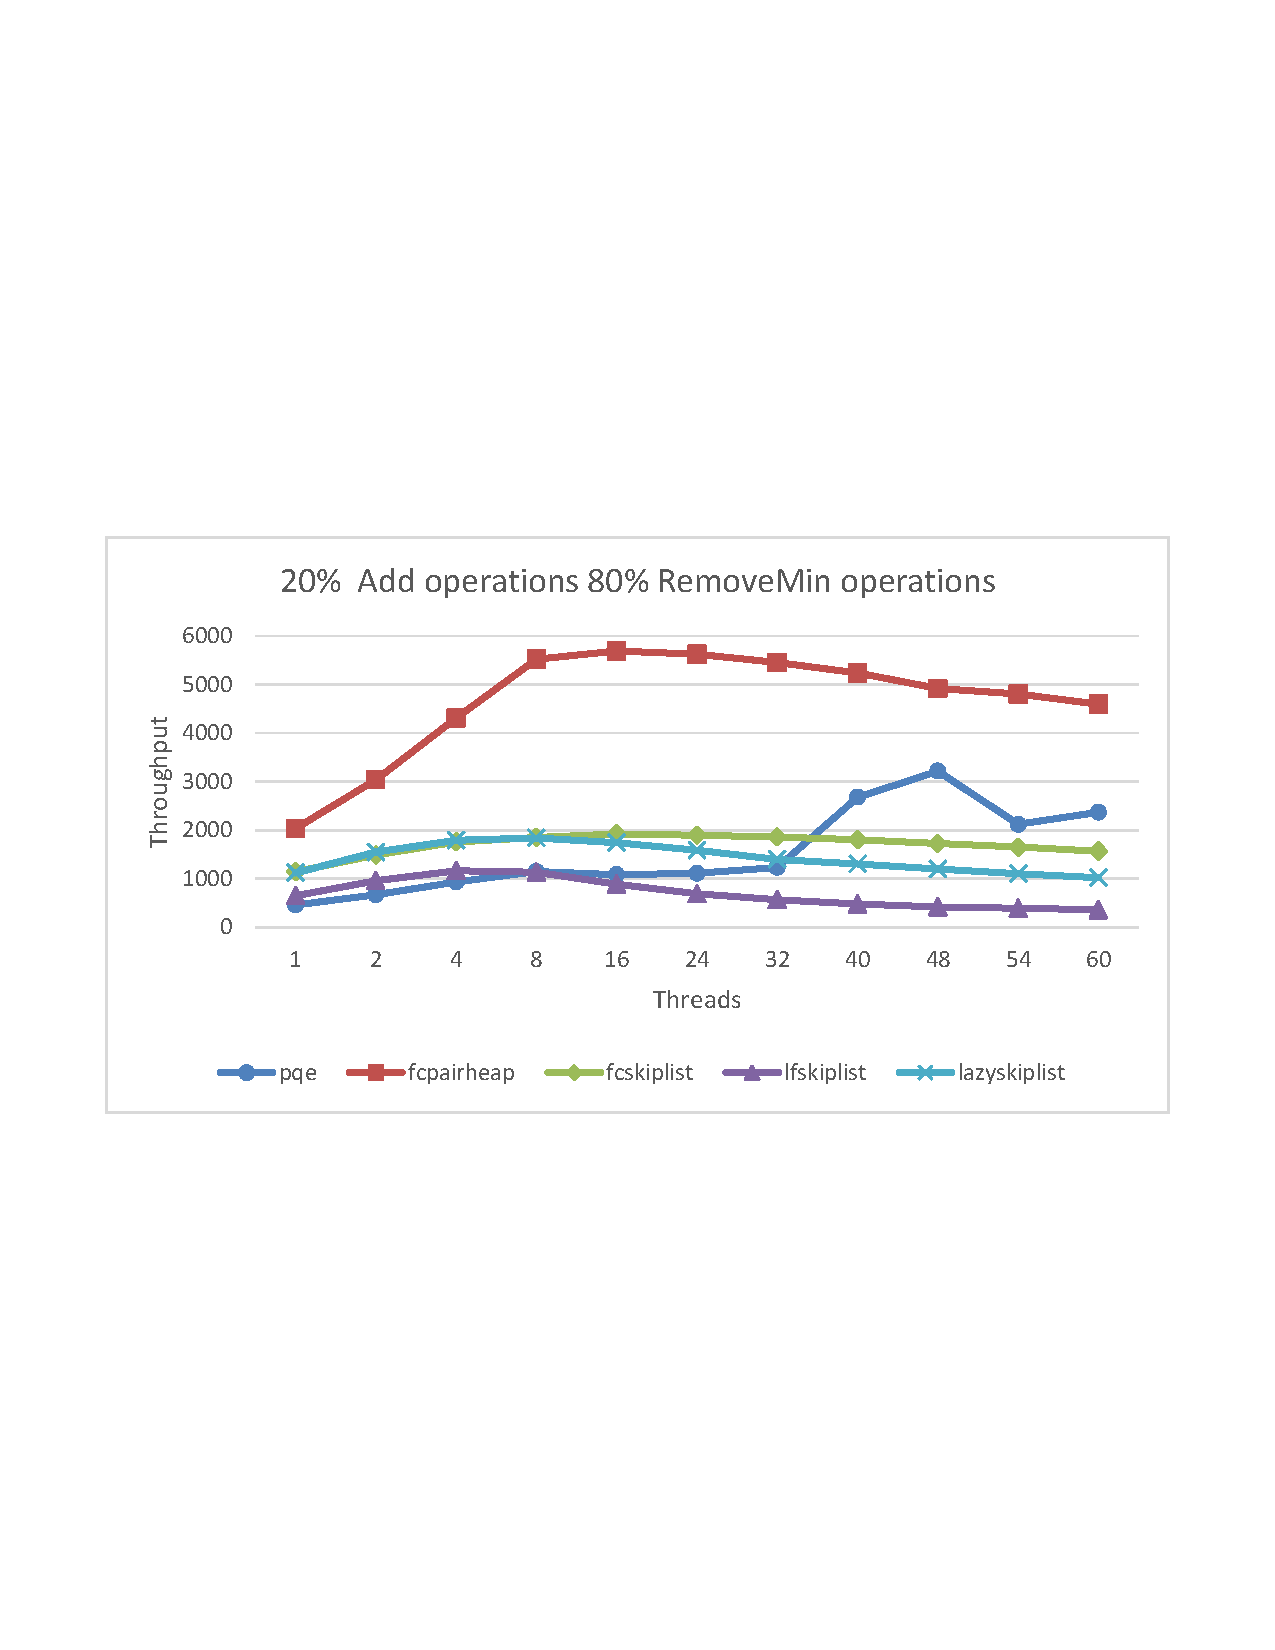
\includegraphics[width=\linewidth]{graphics/sparc-20-80.pdf}
		\caption{Priority queue performance with 20\% \texttt{add()}s, 80\% \texttt{removeMin()}s \cite{calciu_adaptive_2014}.}
		\label{fig:sparc_20}
	\end{minipage}
\end{figure}

\subsubsection{Head-Moving Operations Overhead}

\begin{figure}[htb]
	\centering
	\begin{minipage}[b]{.495\textwidth}
		\centering
		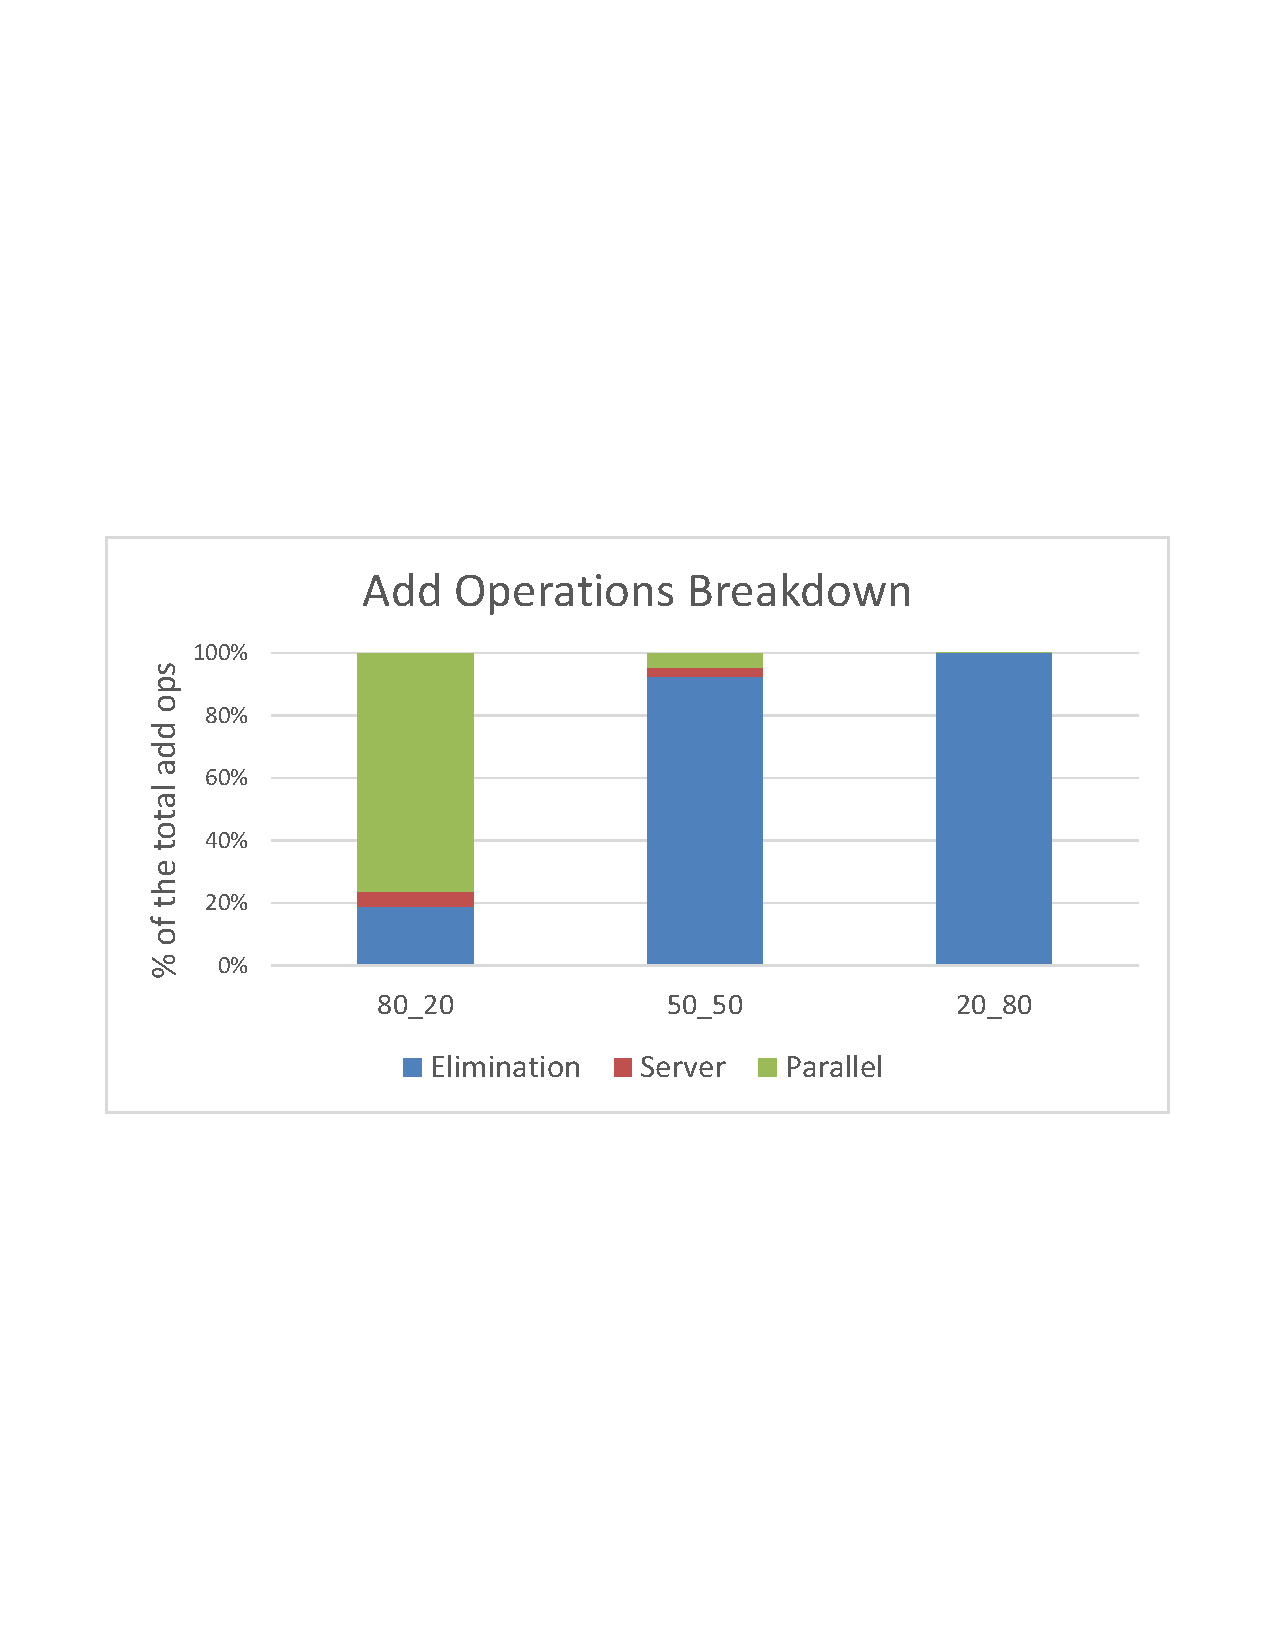
\includegraphics[width=\linewidth]{graphics/sparc-add-brk.pdf}
		\caption{\texttt{add()} work breakdown \cite{calciu_adaptive_2014}.}
		\label{fig:sparc_add}
	\end{minipage}
	\hfill%
	\begin{minipage}[b]{.495\textwidth}
		\centering
		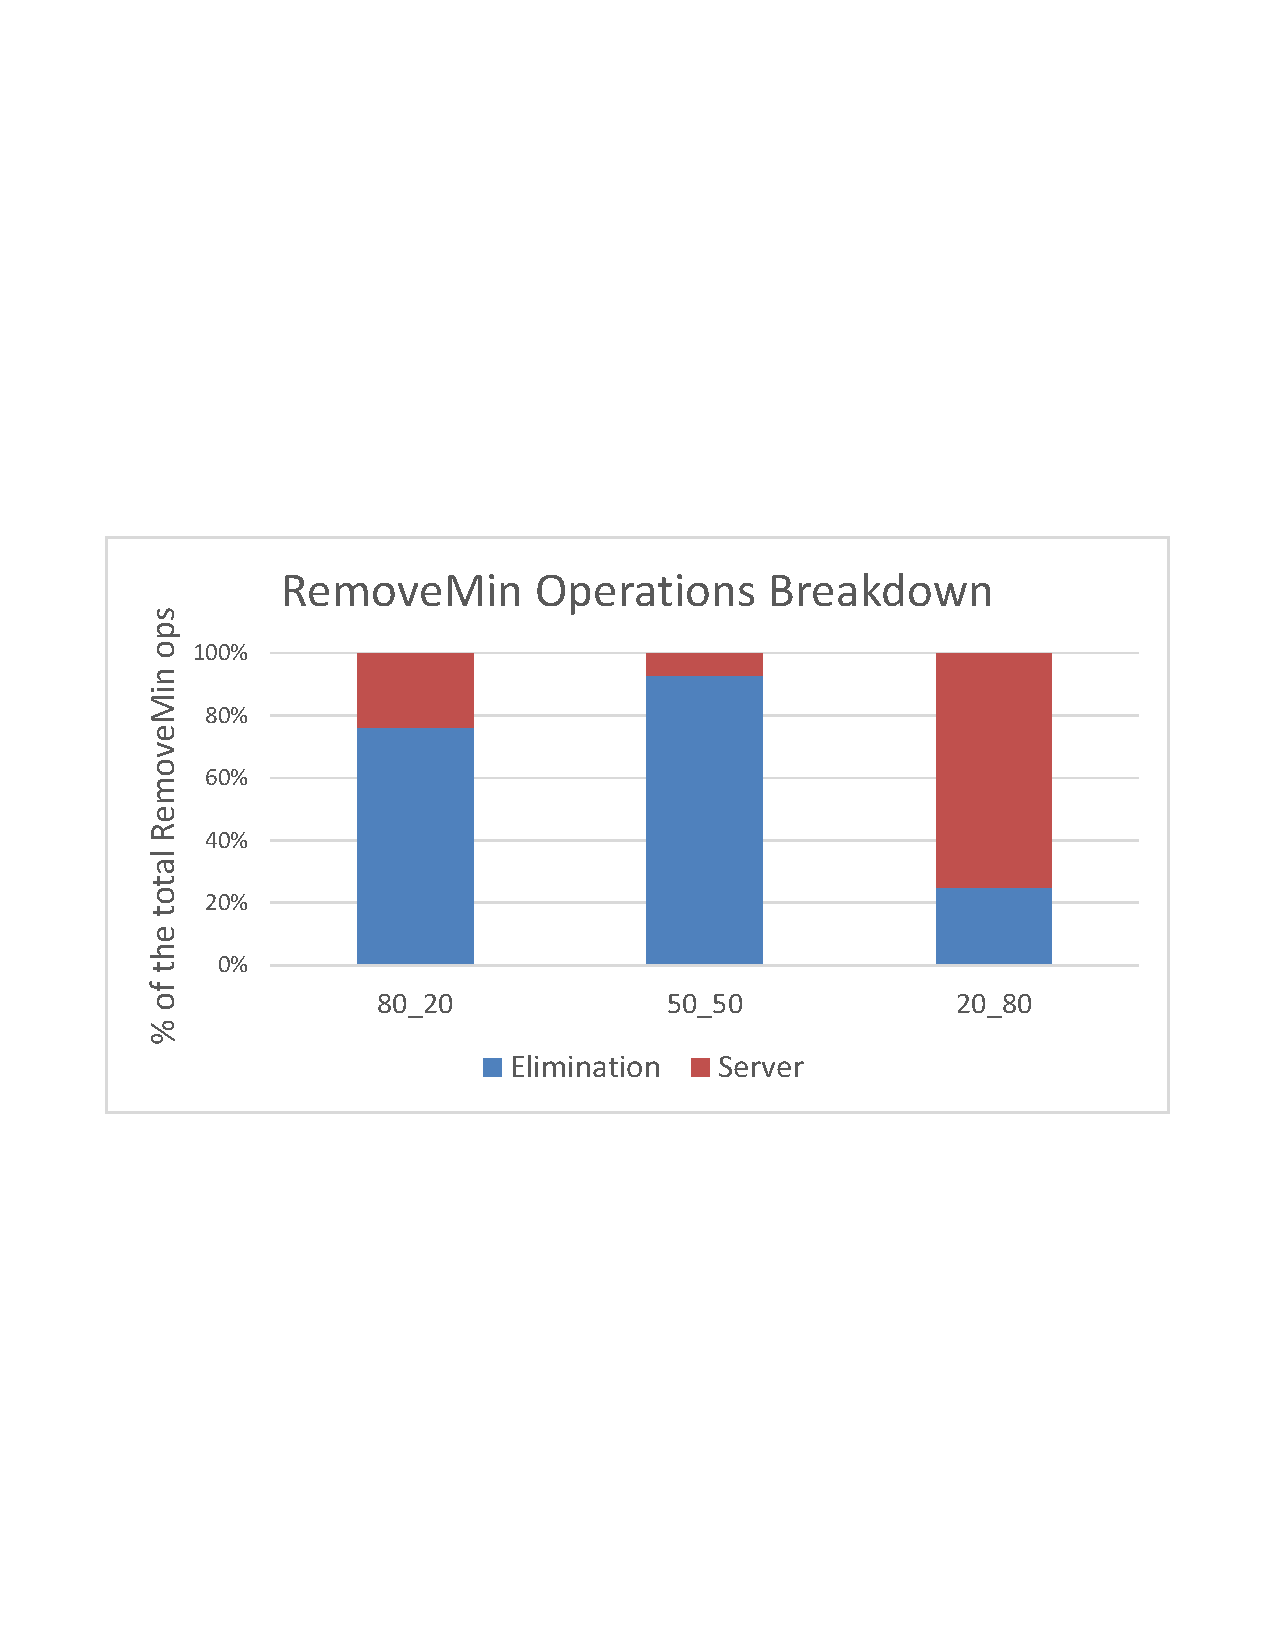
\includegraphics[width=\linewidth]{graphics/sparc-rem-brk.pdf}
		\caption{\texttt{removeMin()} work breakdown \cite{calciu_adaptive_2014}.}
		\label{fig:sparc_rem}
	\end{minipage}
\end{figure}

\subsection{Hardware Transactional Memory Implementation}

To evaluate the performance of the hardware transactional memory implementation a Intel Core i7-4770 based computer was used. The four cores run at 3.4~GHz and provide two hardware threads each.

, with hardware transactions enabled (restricted transactional memory - RTM),
running at . There are 8GB of RAM shared across the machine and each core has a 32KB L1
cache. Hyperthreading was enabled on our machine so we collected results using all 8 hardware threads.
Hyperthreading causes resource sharing between the hyperthreads, including L1 cache sharing, when running
with more than 4 threads, thus it can negatively impact results, especially for hardware transactions. We
did not notice a hyperthreading effect in our experiments. We used the GCC 4.8 compiler with support for
RTM and optimizations enabled (-O3).

\subsubsection{Aborted Transaction Overhead}

\subsection{Comparison with succeeding papers}

\citeauthor{braginsky_cbpq:_2016} claim in their paper that they implemented a high performing parallel priority queue. They used the original sourcecode by \citeauthor{calciu_adaptive_2014} for conducting their evaluation.

\begin{figure}[htb]
	\centering
	\begin{minipage}[b]{.7\textwidth}
		\centering
		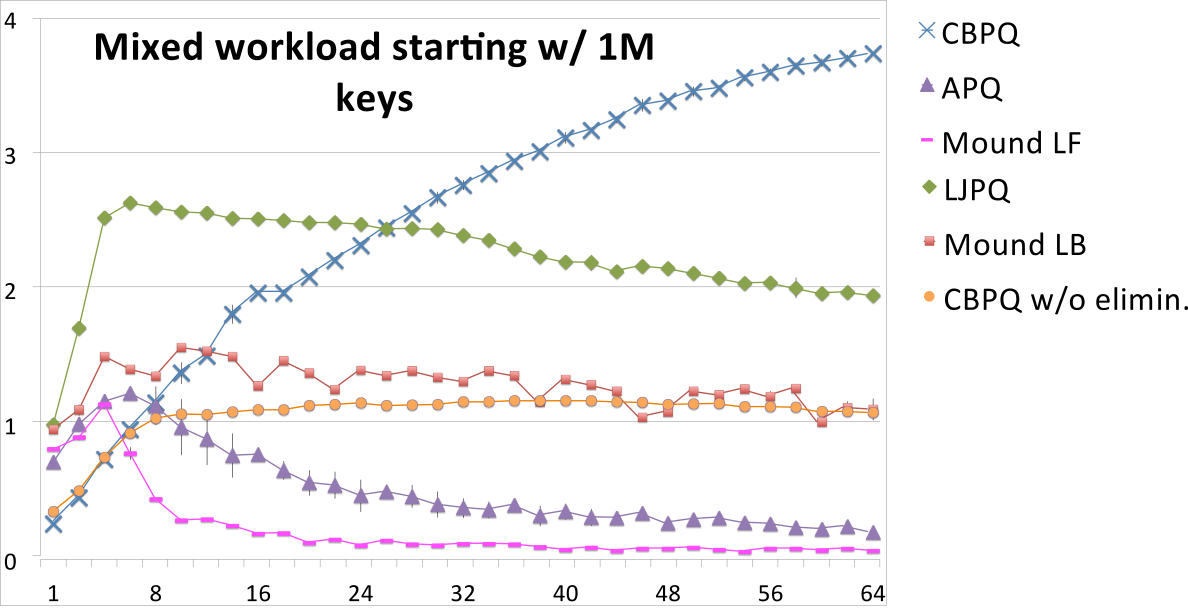
\includegraphics[width=\linewidth]{graphics/cbpq_50add_50.png}
		\caption{Priority queue performance with 50\% \texttt{add()}s, 50\% \texttt{removeMin()}s \cite{braginsky_cbpq:_2016}.}
		\label{fig:cbpq_50}
	\end{minipage}
	\hfill%
	\begin{minipage}[b]{.495\textwidth}
		\centering
		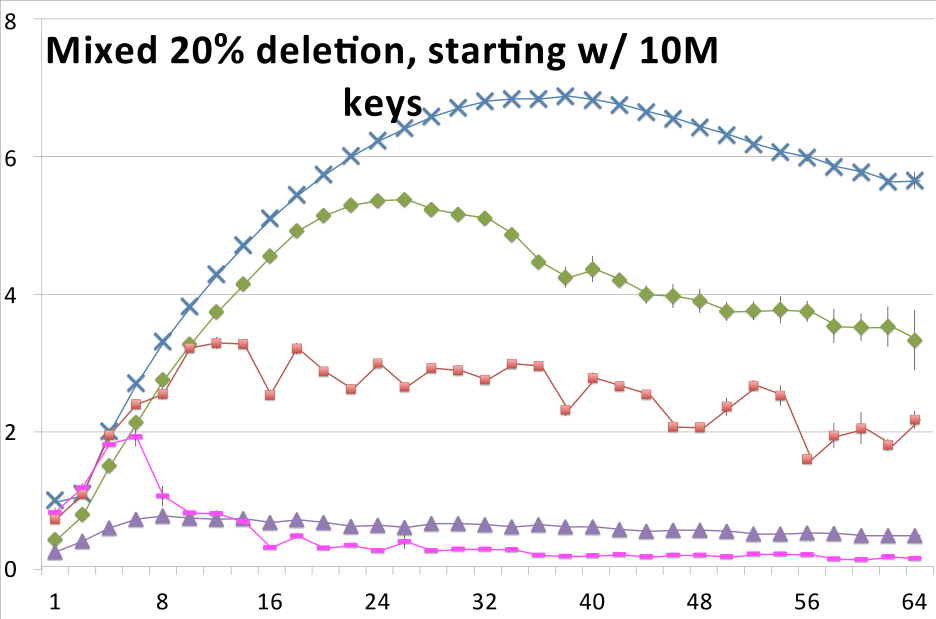
\includegraphics[width=\linewidth]{graphics/cbpq_80add_20.png}
		\caption{Priority queue performance with 80\% \texttt{add()}s, 20\% \texttt{removeMin()}s \cite{braginsky_cbpq:_2016}.}
		\label{fig:cbpq_80}
	\end{minipage}
	\begin{minipage}[b]{.495\textwidth}
		\centering
		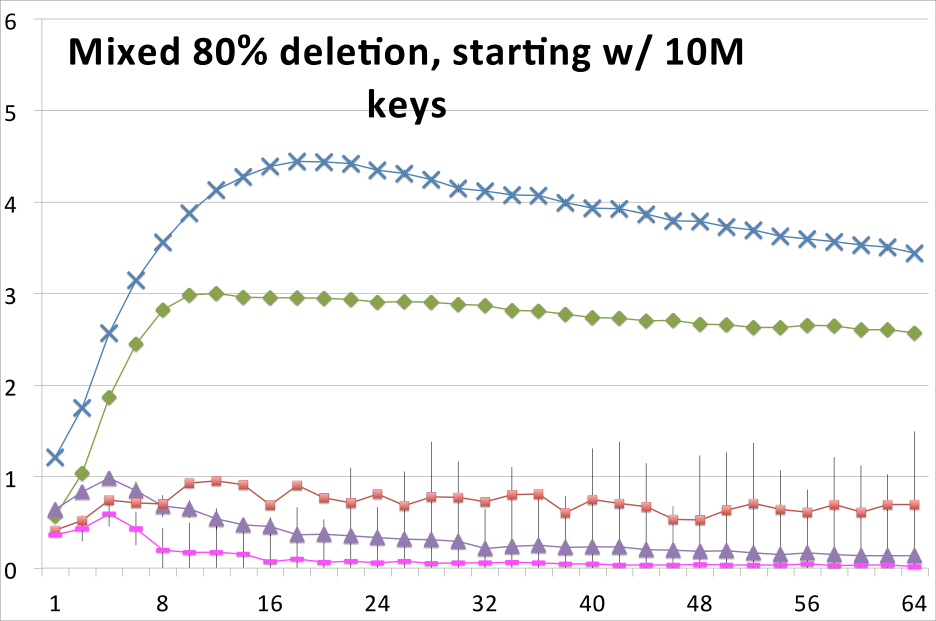
\includegraphics[width=\linewidth]{graphics/cbpq_20add_80.png}
		\caption{Priority queue performance with 20\% \texttt{add()}s, 80\% \texttt{removeMin()}s \cite{braginsky_cbpq:_2016}.}
		\label{fig:cbpq_20}
	\end{minipage}
\end{figure}

The evaluation environment used differs though from the one used by \citeauthor{calciu_adaptive_2014}

C++ and compiled with a -O3 optimization level

\cite{braginsky_cbpq:_2016, } way better (used original code of this paper)

algorithm doesn't seem to scale much on multi socket machine, significant performance drop after useage of

AMD Opteron (TM) 6272
16-core processors, overall 64 threads. The machine was operated by Linux OS
(Ubuntu 14.04)

